\documentclass[pageno]{jpaper}
%\newcommand{\iscasubmissionnumber}{117}

\usepackage[normalem]{ulem}
\usepackage{booktabs}
\usepackage{mathtools}
\usepackage{ragged2e}
\usepackage{rotating}
\usepackage{array}
\usepackage{grffile}

\usepackage{epsfig}
\usepackage{float}
\usepackage{wrapfig}
\usepackage{setspace}
\usepackage{multirow}
\usepackage{graphicx}
%\usepackage{paralist}
%\usepackage{capt-of}

\usepackage{color}
\usepackage{xcolor,colortbl}
\usepackage{chngpage}
\usepackage{enumitem}
\usepackage{enumerate}
\usepackage{amsmath,relsize}
\usepackage[justification=centering]{caption}
\usepackage{tabu}
\usepackage{stmaryrd} % short right arrow

\usepackage{listings}
\usepackage[makeroom]{cancel}


\usepackage{amssymb}% http://ctan.org/pkg/amssymb
\usepackage{pifont}% http://ctan.org/pkg/pifont
\usepackage[nomargin,inline,draft]{fixme}
\newcommand{\cm} {\clap{\small\ding{51}}\small\hphantom{--}}
\newcommand{\cmi}{\clap{\small\ding{51}-}\small\hphantom{--}}%
%\newcommand{\xm} {\clap{\ding{55}}\hphantom{--}}
\newcommand{\xm} {\clap{\small}\small\hphantom{--}}

\newcommand{\Forall}{\displaystyle\mathop\mathlarger{\mathlarger{\mathlarger{\forall}}} } 

%\newcommand{\cm} {{Y}}%
%\newcommand{\cmi}{{P}}%
%\newcommand{\xm} {{}}%


\usepackage{tikz,array}
\usetikzlibrary{calc}

%\newcommand*\circled[1]{\tikz[baseline=(char.base)]{
%            \node[shape=circle,draw,inner sep=2pt] (char) {#1};}}

%\newcommand*\ccircled[1]{\tikz[baseline=(char.base)]{
%            \node[shape=circle,draw,inner sep=2pt] (char) {#1};}}

\tikzstyle{every node}=[font=\footnotesize]

\newcommand{\hcancel}[5]{%
    \tikz[baseline=(tocancel.base)]{
        \node[inner sep=0pt,outer sep=0pt] (tocancel) {#1};
        \draw[black] ($(tocancel.south west)+(#2,#3)$) -- ($(tocancel.north east)+(#4,#5)$);
    }%
}%

\newcommand*\circled[1]{\tikz[baseline=(char.base)]{
            \node[shape=circle,draw,inner sep=0.5pt, minimum size=0.24cm] (char) {#1\vphantom{H}};}}

\newcommand*\ccircled[1]{\hcancel{\tikz[baseline=(char.base)]{
            \node[shape=circle,draw,inner sep=0.4pt, minimum size=0.24cm] (char) {#1\vphantom{H}};}}{-1pt}{1pt}{1pt}{-1pt} }


\begin{document}
\title{
\vspace{-0.15in}
Benchmarking Inter-Process Communication Mechanisms
\vspace{-0.15in}
}



\author{Vinay Gangadhar \\ gangadhar@wisc.edu \\ University of Wisconsin Madison \and Bhuvana Kakunoori \\ kakunoori@wisc.edu \\ University of Wisconsin Madison}

\date{}
\maketitle

%\thispagestyle{empty}
\begin{abstract} \vspace{0.05in} 



In this paper, we benchmark three important inter processor communication (IPC) mechanisms, namely pipes, sockets and bounded buffer shared memory. We measure and compare the performance of these mechanisms for varying input buffer sizes, starting with 4k and increasing up to 512k bytes. We are interested in understanding the scalability and suitability of these mechanisms for different input parameters. In order to do this, we design experiments and evaluate timing tools that can help us measure latency and throughput for each of the above mentioned mechanisms. 

\end{abstract}

\section{Introduction}\label{sec:intro}

\fixme{introduction here}

IPC mechanisms enable multiple processes in a system to communicate with each other. Different methods can be used for this purpose, depending on the application requirements and the process runtime environment. 
Pipes
Pipes provide a unidirectional communication channel between 2 processes. The data written on the write end of the pipe is buffered by the kernel until it is read from the other end of the pipe.
Sockets
< Enter brief description here>
Shared Memory
Shared memory provides the communicating processes, a simultaneous access to a section of memory. Synchronization primitives are used to coordinate access to the shared region. 

\if 0
\begin{figure}
  \includegraphics[width=\linewidth]{figs/first-fig.pdf}
  \caption{Energy/Performance for BERET/C-Cores/Revolver/Composite Cores (bigLITTLE) \newline 
           \textnormal{\small (See section~\ref{sec:methodology} for methodology)} }
  \label{fig:existing}
\end{figure}
\fi


\paragraph{Contributions}
\begin{itemize}
\item \textbf {Contributions here},
\end{itemize}

\paragraph{Paper Organization}
first ($\S$\ref{sec:overview}), and subsequently describe the
evalaution ($\S$\ref{sec:eval}) and results($\S$\ref{sec:res}).
Finally conclusion($\S$\ref{sec:conc}).


 
%\input{analysis}
\section{Overview}\label{sec:overview}



\fixme{Inter-Process Communication - some 2 lines}

\paragraph{Pipes}

\paragraph{Sockets}

\paragraph{Shared Memory}


%\input{architecture}
%\input{compiler}
%\input{related}
%\input{methodology}
\section{Evaluation}\label{sec:eval}

%\subsection*{\ref{itm:pipes} 

\section{Results}\label{sec:res}

%\subsection*{\ref{itm:pipes} 


\begin{figure}
  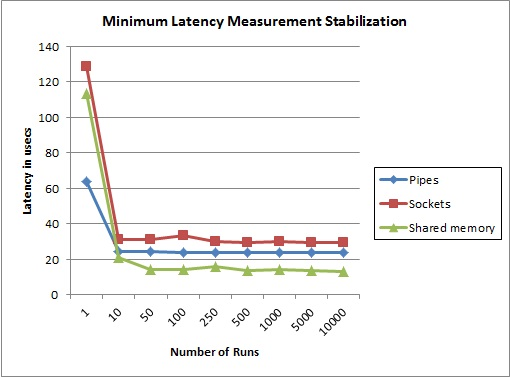
\includegraphics[width=\linewidth]{graphs/jitter.jpg}
  \caption{Jitter} 
  \label{fig:jitter}
\end{figure}

\begin{figure}
  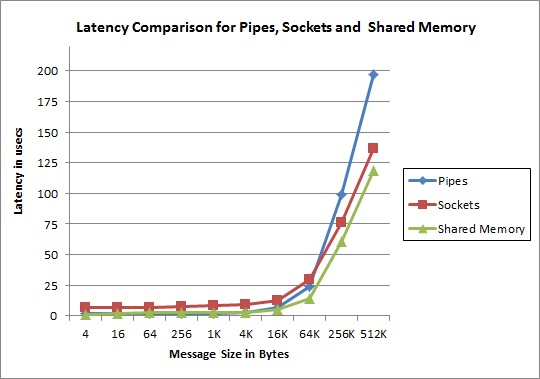
\includegraphics[width=\linewidth]{graphs/lat.jpg}
  \caption{Latency} 
  \label{fig:lat}
\end{figure}

\begin{figure}
  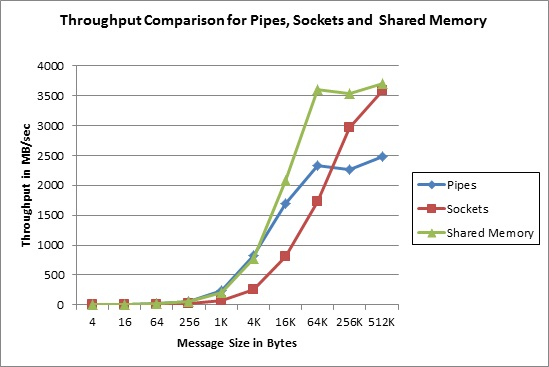
\includegraphics[width=\linewidth]{graphs/tpt.jpg}
  \caption{Throughput} 
  \label{fig:tpt}
\end{figure}



\section{Conclusion}\label{sec:conc}

\fixme{concluding remarks}




\bstctlcite{bstctl:etal, bstctl:nodash, bstctl:simpurl}
\bibliographystyle{IEEEtranS}
\bibliography{main}

\end{document}
